\documentclass[12pt,a4paper]{article}
\usepackage[utf8]{inputenc}
\usepackage[czech]{babel}
\usepackage[T1]{fontenc}
\usepackage{amsmath}
\usepackage{amsfonts}
\usepackage{amssymb}
\usepackage{graphicx}
\usepackage{titlesec}
\usepackage[left=2cm,right=2cm,top=2cm,bottom=2cm]{geometry}
\usepackage{indentfirst}
\usepackage{listings}
\usepackage{color}
\usepackage{array}
\usepackage[]{algorithm2e}

%Pravidlo pro řádkování
\renewcommand{\baselinestretch}{1.2}

%Pravidlo pro začínání kapitol na novém řádku
\let\oldsection\section
\renewcommand\section{\clearpage\oldsection}

%Formáty písem pro nadpisy (-změněno na bezpatkové \sffamily z původního \normalfont
\titleformat{\section}
{\sffamily\Large\bfseries}{\thesection}{1em}{}
\titleformat{\subsection}
{\sffamily\large\bfseries}{\thesubsection}{1em}{}
\titleformat{\subsubsection}
{\sffamily\normalsize\bfseries}{\thesubsubsection}{1em}{}

%Nastavení zvýrazňování kódu v \lslisting
\definecolor{mygreen}{rgb}{0,0.6,0}
\definecolor{mygray}{rgb}{0.5,0.5,0.5}
\lstset{commentstyle=\color{mygreen},keywordstyle=\color{blue},numberstyle=\tiny\color{mygray}}

\author{Jan Šmejkal}

\begin{document}

%-------------Úvodni strana---------------
\begin{titlepage}


\includegraphics[width=50mm]{img/FAV.jpg}
\\[160 pt]
\centerline{ \Huge \sc KIV/PRO - Programátorské Strategie}
\centerline{ \huge \sc Semestrální práce}
\\[12 pt]
{\large \sc
\centerline{\LARGE{KLC - Kiwi Legible Caesar}}
\centerline{(Kiwi Čitelná Caesarova šifra)}
\centerline{\small{Implementace algoritmu Nová modifikace kryptografické metody Césarovy Šifry}}
}


{
\vfill 
\parindent=0cm
\textbf{Jméno:} Štěpán Ševčík\\
\textbf{Osobní číslo:} A13B0443P\\
\textbf{E-mail:} kiwi@students.zcu.cz\\
\textbf{Datum:} {\large \today\par} %datum

}

\end{titlepage}

%------------------Obsah-------------------
\newpage
\setcounter{page}{2}
\setcounter{tocdepth}{3}
\tableofcontents
%------------------------------------------

%--------------Text dokumentu--------------

\section{Úvod}
Kryptografie je věda, která se zabývá navrhováním metod, které umožňují přenos informací takovým způsobem, že jediná osoba schopná získání těchto informací je míněný příjemce.
V raných dobách byla kryptografie prováděna manuálními technikami. Od té doby se základní koncept kryptografie téměř nezměnil s výjimkou řady vylepšení provedení a její samotné implementace. \newline
Způsoby vytváření tajné zprávy lze rozdělit do dvou základních metodik, kterými jsou Kryptografie a Steganografie. Zpráva v podobě prostého textu lze skrýt jednou z těchto metodik. Pomocí Steganografie lze docílit skrytí existence dané zprávy zatímco Kryptografie se snaží o snížení srozumitelnosti pomocí různých transformací této zprávy.\newline
Kryptografie je spíše mířená na vytvoření šifry zatímco Steganografie se více zaobírá skrývání existence zprávy. Nicméně obě metodiky mají stejný cíl - zatajení zprávy. Ukazuje se ale, že šifry vytvořené metodami Kryptografie lze často prolomit další osobou nebo kryptoanalytikem. Toto je s největší pravděpodobností způsobeno tím, že nečitelná zpráva vzbuzuje podezření, že obsahuje skrytý význam. Toto podezření je startovací signál pro kryptoanalytika, který začíná zkoušet aplikovat metody pro dešifrování. Jednoduchá forma Kryptografie, která je ale časově náročná, je taková, která uspořádává slov nebo písmen ve zdánlivě neškodném textu, které tvoří samotnou zprávu. V tomto článku autoři vytváří modifikaci Césarovy šifry, aby byl výsledek čitelný a tím pádem aby kryptoanalytik nebyl podezřívavý a nesnažil se šifru prolomit\cite{purnama93}.
\subsection{Kryptografie}
Kryptologie není nijak nová oblast - existuje již přes 2000 let a Kryptografie je podoblast Kryptologie. Název Kryptologie se skládá z řeckých slov \textbf{cryptos} (=skryté) a \textbf{logos} (=věda), tedy Kryptologie je doslova věda zabývající se skrýváním.
V Kryptografii se původní zprávě říká prostý text a zakódované zprávě se říká šifra. Procesu převodu textu na šifru se říká šifrování a převodu šifry na text se říká dešifrování. Do těchto procesů je často zakomponován šifrovací klíč a celý proces přenosu šifrované informace je znázorněn na Obrázku \ref{img:ciphertextTransfer}.\cite{kiwi16}

\begin{figure}[h]
\center
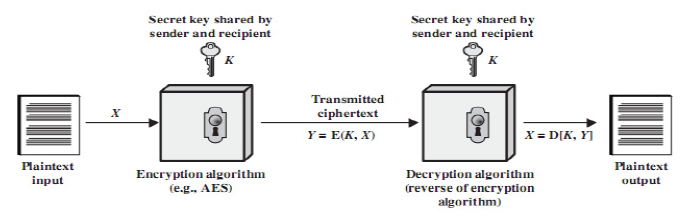
\includegraphics[width=0.9\textwidth]{img/ciphertextTransfer.png}
\caption{Grafické znázornění přenosu šifrované informace.}
\label{img:ciphertextTransfer}
\end{figure}

\section{Algoritmus}
\subsection{Standardní Caesarova Šifra}
Šifrování a dešifrování standardní Caesarovou šifrou lze popsat jednoduchým vzorcem.
\begin{equation}
c = E(k, p) = p + k mod26
p = D(k, c) = c - k mod26
\end{equation}
Kde znaky představují:
\begin{tabular}{ll}
$c$ = Znak šifry & $p$ Znak prostého textu \\
$b_k$ = klíč / číslo řádky 
\end{tabular} \cite{kiwi16}. \\
\subsection{Modifikace Caesarovy šifry pro čitelnost}
Modifikovaný algoritmus definuje množiny znaků, ve kterých znak vždy zůstává přes průběh šifrování i dešifrování. Znaky, které nejsou v definovaných množinách zůstávají nenahrazené.

Například tedy, pokud jsou definované množiny znaků \texttt{[ \{ABC\}, \{DE\} ]}, počet možností zakódování libovolného slova je 6\cite{kiwi16}. Možnosti zakódování slova BEADS jsou znázorněny v Tabulce \ref{tab:beads}.\\
\begin{table}[h]
\caption{Ukázka zakódování slova BEADS na jednoduchých množinách znaků.}
\label{tab:beads}
\center
\begin{tabular}{|c|c||c|c|}
\hline
\textbf{Klíč} & \textbf{Šifra} & \textbf{Klíč} & \textbf{Šifra}\\ \hline
0 & BEADS & 3 & BDAES \\ \hline
1 & CDBES & 4 & CEBDS \\ \hline
2 & AECDS & 5 & ADCES \\ \hline
\end{tabular}
\end{table}

Toto je případ, kdy čitelnost šifry není zaručena. Nečitelnost šifry vyplývá ze špatné volby množin znaků pro nahrazování.

V jednoduché konstrukci algoritmu potom zavádíme pravidla pro tvorbu množin znaků:
\begin{itemize}
\item Samohlásky \textbf{AIUEO} budou nahrazeny pouze samohláskami.
\item Souhlásky \textbf{BCDFGHJKLMNPQRSTVWXYZ} budou nahrazeny pouze souhláskami.
\end{itemize}
Pozn.: Tato pravidla je při adaptaci na konkrétní jazyk třeba rozšířit a/nebo upravit ale pro všeobecnou implementaci jsou dostačující.

\section{Algoritmus KLC}
Tento článek se zabývá implementací algoritmu Kiwi Legible Caesar, který doplňuje výše zmíněný algoritmus, ve skriptovacím jazyce JavaScript. Tím pádem je tato implementace extrémně přenositelná a jednoduše spustitelná - postačuje k tomu libovolný interpret jazyka JavaScript, například moderní webový prohlížeč.

Algoritmus využívá množina unikátních znaků, které definují způsob generování způsobů zašifrování slova. Pro tyto množiny platí že:
\begin{itemize}
\setlength\itemsep{0.1em}
\item Pokud se množiny skládají ze stejných znaků, generují stejné množiny způsobů zašifrování slova, pouze v různých pořadích.
\item Počet způsobů zašifrování slova je určen jakožto nejmenší společný násobek (neboli Lowest Common multiple, tedy lcm) velikostí těchto množin.
\item Soubor těchto množin a počet způsobů zašifrování slova tvoří takzvaný "kodek".
\end{itemize}

Algoritmy pro šifrování a dešifrování používají pro posunutí slova stejný algoritmus s různým posunem znaků. Posunutí slova je implementována Algoritmem \ref{alg:shiftWord}. \\ 
\fbox{\begin{algorithm}[H]
\SetAlgorithmName{Algoritmus}{}
 \KwData{$[a_1, a_2, ..., a_n], offset, [charset_1, charset_2, ..., charset_m]$}
 \KwResult{$[b_1, b_2, ..., b_n]$}
%initialisation;
 \For{$i = 1; i \leq n; i++;$}{
   $charset_{a_i} = find\_charset\_containing(a_i)$\;
  \eIf{$charset_{a_i}$ does not exist}{
    $b_i := a_i$\;
  }{
    $charset\_size := size(charset_{a_i})$\;
    $b_i := (a_i + offset) mod_{charset\_size}$\;
  }
 }
 \caption{Posunutí slova}
 \label{alg:shiftWord}
\end{algorithm}}

\bigskip \noindent
Pro správné fungování algoritmů šifrování a dešifrování je nutné, aby množiny posouvaných znaků obsahovaly unikátní znaky v rámci množiny i mezi sebou.
\newpage
\subsection{Šifrování}
Algoritmus šifrování probíhá v krocích, kde se každé slovo šifruje zvlášť. funkce
Průběh šifrování je vizualizován Algoritmem \ref{alg:encryptAll}. 

Funkce get\_key($word_i$) generuje všechny možné varianty pro zašifrování slova a nechává uživatele zvolit žádnou šifru. Pro testování algoritmu je výběr nahrazen generováním pseudonáhodného čísla odpovídající způsobu zašifrování konkrétního slova. \\
\fbox{\begin{algorithm}[H]
\SetAlgorithmName{Algoritmus}{}
 \KwData{$[word_1, word_2, ..., word_n], [charset_1, charset_2, ..., charset_m]$}
 \KwResult{$[cipher_1, cipher_2, ..., cipher_n], [key_1, key_2, ..., key_3]$}
%initialisation;
 \For{$i := 1; i \leq n; i++;$}{
  $key_i :=$ get\_key($word_i$)\;
  $cipher_i :=$ shift\_word($word_i, key_i$)\;
 }
 \caption{Zašifrování množiny slov}
 \label{alg:encryptAll}
\end{algorithm}}

\subsection{Dešifrování}
Algoritmus dešifrování probíhá stejně jako algoritmus šifrování s tím rozdílem, že je použit takzvaný 'zpětný chod' při posouvání slova. Dále odpadá potřeba pro zobrazení možných způsobů dešifrování protože je způsob jednoznačně určen doprovázejícím klíčem. \\
\fbox{\begin{algorithm}[H]
\SetAlgorithmName{Algoritmus}{}
 \KwData{$[cipher_1, cipher_2, ..., cipher_n], [key_1, key_2, ..., key_3], [charset_1, charset_2, ..., charset_m]$}
 \KwResult{$[word_1, word_2, ..., word_n]$}
 charset\_sizes = calc\_sizes($charset_1, charset_2, ..., charset_m$)\;
 variations\_count = lcm(charset\_sizes)\;
 \For{$i := 1; i \leq n; i++;$}{
  $key_i :=$ get\_key($word_i$)\;
  $word_i :=$ shift\_word($cipher_i, variations\_count - key_i$)\;
 }
 \caption{Rozšifrování množiny slov}
 \label{alg:decryptAll}
\end{algorithm}}

\subsection{Adresářová struktura implementace}
Adresářová struktura odpovídá jednoduché webové prezentaci:
\texttt{index.html} obsahuje šablonu uživatelského rozhraní, v adresáři \texttt{css}jsou obsaženy konkrétní styly šablony. Adresář \texttt{vendor} obsahuje styl Bootstrapu a skripty jQuery, které urychlují vývoj uživatelského rozhraní.

Veškerá logika je umístěna v adresáři \texttt{js}, konkrétně v souborech \texttt{Codec.js}, \texttt{CodesetSupplier.js} a \texttt{main.js}, který obsahuje napojení na uživatelské rozhraní.

\section{Testování implementace algoritmu KLC}
Pro porovnávání byly vytvořeny tři kodeky různých velikostí:
\begin{enumerate}
\setlength\itemsep{0.0em}
\item \textbf{Celá abeceda}, tvořený z množin znaků "aeiou" a "bcdfghjklmnpqrstvwxyz" o velikostech 5 a 21 znaků. Počet způsobů zašifrování slova je tedy 105.
\item \textbf{Originál}, kodek vytvořený podle původního článku. Skládá se z množin "aoeiu" a "bdjmprlscfhktw" o velikostech 5 a 16 a počet způsobů vytvoření slova je 70.
\item \textbf{Abeceda bez X} je odlehčená varianta prvního kodeku. Velikosti množin jsou 5 a 20 a tedy počet způsobů zašifrování slova je 20.
\end{enumerate}

Algoritmus byl spouštěn s těmito kodeky postupně na testovacích textech před-generenovaných pomocí \textit{Lorem Ipsum} algoritmu na serveru http://cs.lipsum.com/. Testovací množiny obsahovaly 68646, 137290 a 205936 slov.

Uživatelský vstup byl simulován, tj místo čekání na vstup bylo generováno pseudonáhodné číslo v rozsahu <0; [počet variací kodeku]>.
Výsledné časy znázorněny v Tabulce \ref{tab:results} představují aritmetické průměry z pěti měření.

\subsection{Výsledky testování}

Barevně oddělené páry sloupců představují variantu algoritmu, generující pro každé slovo N šifer, kde N je číslo uvedené v prvním řádku, druhý řádek určuje, algoritmus pro daný sloupec a následující řádky obsahují dobu výkonu algoritmu pro počet slov stanovený ve druhém sloupci.

\begin{table}[h]
\center
\caption{Tabulka výsledných časů variant algoritmů šifrování a dešifrování na různých množinách. Časy jsou uvedeny v milisekundách.}
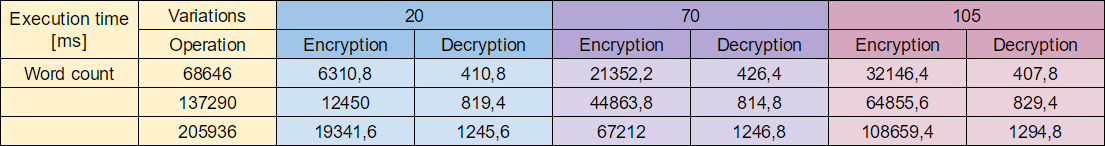
\includegraphics[width=0.9\textwidth]{img/results.png}
\label{tab:results}
\end{table}

\subsection{Poznatky}
\begin{itemize}
\setlength\itemsep{0.0em}
\item Algoritmus dešifrování zpracuje 1000 párů šifra-klíč průměrně za 6.07 milisekund.
\item Algoritmus šifrování(20 šifer) vygeneruje 1000 párů šifra-klíč průměrně za 92.18 milisekund.
\item Algoritmus šifrování(70 šifer) vygeneruje 1000 párů šifra-klíč průměrně za 321.40 milisekund.
\item Algoritmus šifrování(105 šifer) vygeneruje 1000 párů šifra-klíč průměrně za 321.40 milisekund.
\item Z předcházejících poznatků o algoritmu šifrování vyplývá lineární závislost na počtu variant: při generování 1000 párů každá varianta navíc představuje pro algoritmus zhruba 4.62 milisekund
\end{itemize}


\section{Závěr}
Z výsledků lze ověřit, že algoritmus šifrování má lineární časovou závislost na počtu slov a zároveň lineární časovou závislost na počtu generovaných způsobů zašifrování. Algoritmus dešifrování má pouze lineární závislost na počtu slov.

Při testování bylo také ověřeno, že se ve většině případů v množině způsobů zašifrování slova vyskytuje několik čitelných šifer ale také že tyto výsledné šifry jen v ojedinělých případech představovaly skutečná slova definovaná slovníkem spisovných slov.
Pravděpodobnost výskytu platných slov mezi možnými šiframi možná lze zvýšit sestavením vhodného kodeku.
\begin{thebibliography}{9}

\bibitem{purnama93} 
Benni Purnama and A.H. Hetty Rohayani
\textit{New Modified Caesar Cipher Cryptography Method with Legible Ciphertext From a Message to Be Encrypted}. 
Procedia Computer Science, Volume 59, 2015, Pages 195-204

\bibitem{kiwi16}
Štěpán Ševčík
\textit{Nová modifikace kryptografické metody Césarovy Šifry
jejíž výsledná šifra ze vstupní zprávy je čitelný text} (Nepublikovaná semestrální práce).
Západočeská Univerzita v Plzni, Plzeň, Česká Republika.
 
\end{thebibliography}

%------------------------------------------

\end{document}
